\documentclass[12pt]{article}
\usepackage[utf8]{inputenc}
\usepackage[T2A]{fontenc}
\usepackage[english,russian]{babel}
\usepackage{amsmath,amssymb}
\usepackage{graphicx}

\newcommand{\pd}[2]{\frac{\partial #1}{\partial #2}}

\author{Цыбулин Иван}
\title{Математическая модель вентилятора в системе уравнений газовой динамики}

\begin{document}
\maketitle
Рассмотрим одномерные уравнения газовой динамики
\begin{gather*}
\pd{\rho}{t} + \pd{(\rho u)}{x} = 0\\
\pd{\rho u}{t} + \pd{(\rho u^2 + p)}{x} = 0\\
\pd{e}{t} + \pd{(e + p)u}{x} = 0,\\
e = \rho \varepsilon + \frac{\rho u^2}{2}, \quad p = (\gamma - 1) \rho \varepsilon.
\end{gather*}

Вентилятор можно описать с помощью локализованного на расстоянии $\Delta x$ источника импульса и энергии
\begin{gather*}
\pd{\rho}{t} + \pd{(\rho u)}{x} = 0\\
\pd{\rho u}{t} + \pd{(\rho u^2 + p)}{x} = \frac{\Delta p_\text{fan}}{\Delta x}\\
\pd{e}{t} + \pd{(e + p)u}{x} = \frac{\Delta h_\text{fan} u}{\Delta x},
\end{gather*}
однако в такой постановке сложно получить вентилятор, обеспечивающий заданный расход газа в условиях нестационарного течения.

Альтернативным подходом может служить введение некоторой поверхности (внутренней границы), на которой допускается скачкообразное изменение давления, а расход газа через нее контролируется. Этот подход достаточно просто реализовать в случае использования численного метода Годунова для решения уравнений газовой динамики. Для этого необходимо рассмотреть специальную конфигурацию распада разрыва, учитывающую данные требования.

Предположим, что вентилятор располагается на границе между двумя ячейками разностной сетки. Также предположим, что скорость течения через вентилятор существенно меньше скорости звука. Стандартная конфигурация распада произвольного разрыва в газовой динамике предполагает существование трех волн:
левой волны разрежения (ВР) или ударной волны (УВ), контактного разрыва (КР) и правой волны разрежения или ударной волны. Добавим в этот набор элементарных волн стационарный скачок давления (СД). Добавление данного разрыва позволяет наложить еще одно дополнительное ограничение на решение задачи Римана, например, позволяет положить заданной скорость газа на стационарном скачке.

\begin{figure}[!ht]
\centering
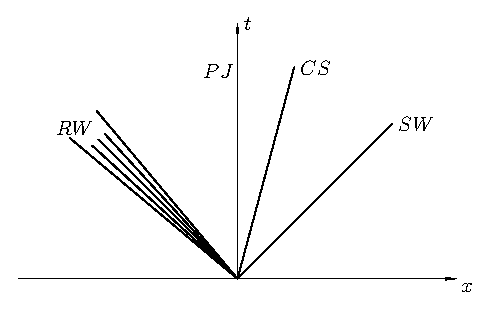
\includegraphics[width=.8\columnwidth]{conf-0.eps}
\caption{Типичная конфигурация распада разрыва на вентиляторе. SW --- ударная волна, CS --- контактный разрыв, PJ --- скачок давления, RW --- волна разрежения}
\end{figure}

\begin{figure}[!ht]
	\centering
	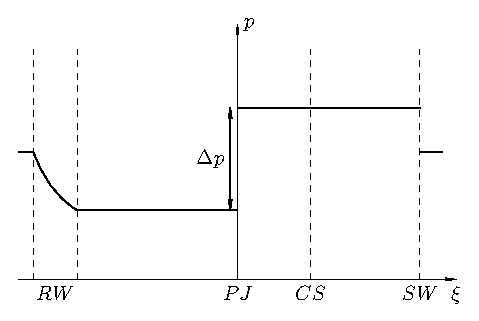
\includegraphics[width=.45\columnwidth]{conf-1.eps} %
%	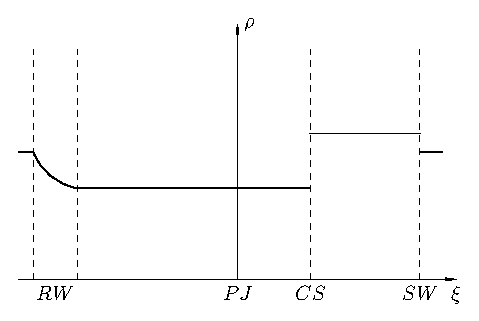
\includegraphics[width=.45\columnwidth]{conf-2.eps}
	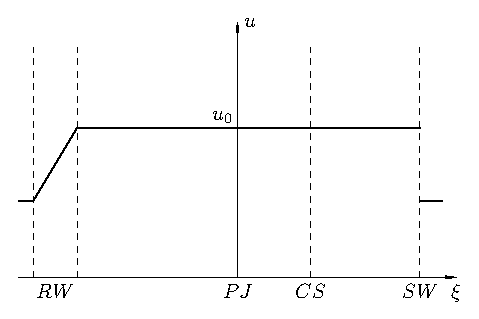
\includegraphics[width=.45\columnwidth]{conf-3.eps} %
	\caption{Изменения параметров $p, u$ по автомодельной переменной $\xi = \frac{x}{t}$}
\end{figure}

Из конфигурации распада видно, что скорость газа за крайними волнами всегда известна и равна $u_0$ --- заданной скорости течения газа через вентилятор. Поскольку параметры газа перед крайними волнами также известны (начальные данные задачи Римана), несложно получить все параметры за крайними волнами. 

Например (см. [Куликовский, Погорелов, Семенов]), для правой ударной волны
\begin{gather*}
v \equiv u_0 - u_2 = \frac{P_2 - p_2}{|m_2|} > 0, \\
|m_2| = \sqrt{\frac{\rho_2}{2} \big[P_2 (\gamma_2 + 1) + p_2 (\gamma_2 - 1)\big]}\\
P_2 = p_2 + \frac{\gamma_2 + 1}{4} \rho_2 v^2 + \frac{v}{4}
\sqrt{16 \gamma_2 \rho_2 p_2 + (\gamma_2 + 1)^2 \rho_2^2 v^2}\\
R_2 = \frac{\rho_2 |m_2|}{|m_2| - \rho_2 v}
.
\end{gather*}
Здесь $\rho_2, u_2, p_2б \gamma_2$ --- параметры справа от первоначального разрыва, $R_2, P_2$ --- плотность и давление за ударной волной.
Для правой волны разрежения
\begin{gather*}
v \equiv u_0 - u_2 = \frac{2c_2}{\gamma_2 - 1} \left[\left(\frac{P_2}{p_2}\right)^{\frac{\gamma_2 - 1}{2\gamma_2}}-1\right] < 0\\
P_2 = p_2 \left(1 + \frac{(\gamma_2 - 1)v}{2c_2}\right)^\frac{2\gamma_2}{\gamma_2 - 1}\\
R_2 = \rho_2 \left(\frac{P_2}{p_2}\right)^{\frac{1}{\gamma_2}}.
\end{gather*}
В звуковом приближении ($|v| \ll c$) оба типа волн дают одинаковый результат
\[
P_2 = p_2 \left(1 + \frac{\gamma_2 v}{c_2}\right), \quad
R_2 = \rho_2 \left(1 + \frac{v}{c_2}\right).
\]

Аналогичные с точностью до симметрии выражения справедливы и для левой стороны. Решение задачи можно проиллюстрировать с помощью $PU$ диаграммы. Также из диаграммы хорошо видно, что такой подход можно обобщить с использованием уравнения состояния вентилятора 
\[
F(\Delta p, u_0) = 0.
\]
\begin{figure}
\centering
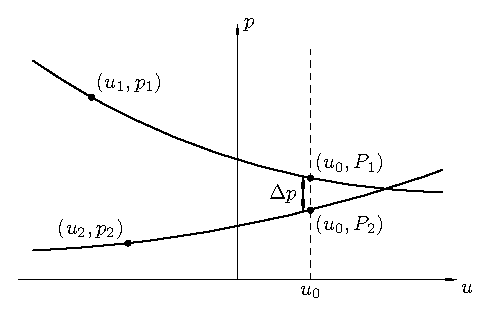
\includegraphics[width=.8\columnwidth]{conf-4.eps}
\caption{$PU$ диаграмма для анализа задачи о распаде разрыва на вентиляторе}
\end{figure}
Контактный разрыв соединяет области со значением плотности $R_1$ слева и $R_2$ справа. В зависимости от знака $u_0$ он находится либо справа ($u_0 > 0$), либо слева ($u_0 < 0$) от стационарного скачка давления.

\end{document}
